ここではSublime Text 2(以下「Sublime」)+GoSublimeの組み合わせをご紹介します。なぜこの組み合わせなのでしょうか?


\begin{itemize}
  \item コード表示の自動化、以下の図の通り\\ 
\begin{figure}[H]
  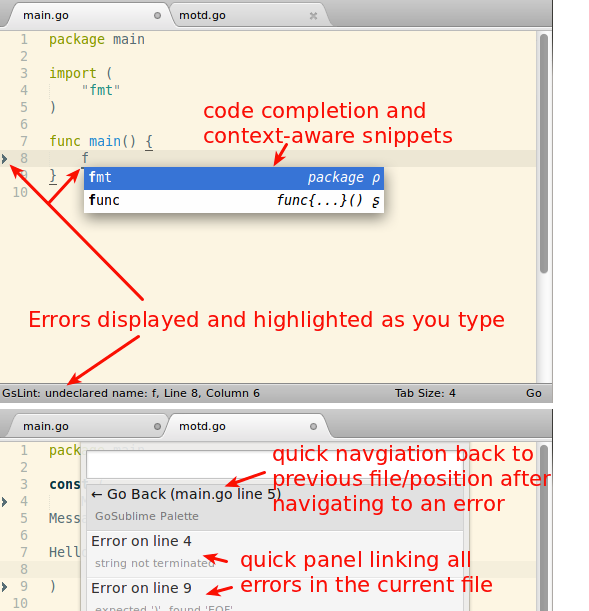
\includegraphics[width=14cm]{1.4.sublime1.png}
   \label{図1.5}
   \caption{sublimeコードの自動化画面}
\end{figure}
  \item 保存した時にはコードが自動的に整形されています。あなたの書いたコードをより美しくGoの標準に合うよう仕上げてくれます。
  \item プロジェクト管理のサポート\\ 
\begin{figure}[H]
  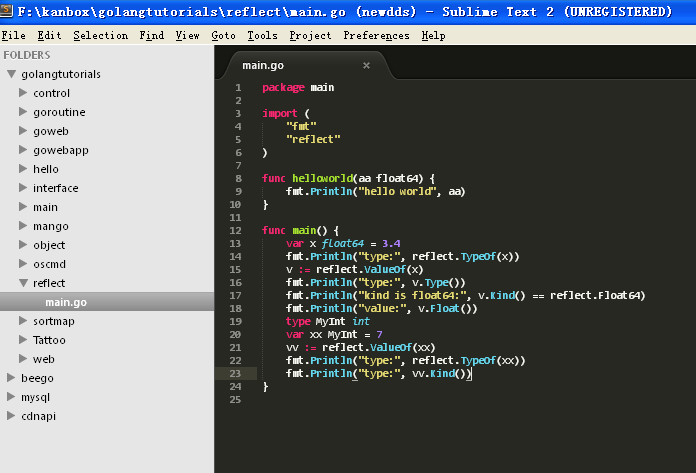
\includegraphics[width=14cm]{1.4.sublime2.png}
   \label{図1.6}
   \caption{sublimeプロジェクト管理画面}
\end{figure}
  \item 文法のハイライトサポート
  \item Sublime Text 2はフリーで使用できます。保存回数が一定の量を超えると購入するかのダイアログが現れるので、継続利用をキャンセルするをクリックします。正式登録版とは何の違いもありません。
\end{itemize}


次はどのようにインストールするかご説明します。Sublimeダウンロードします。

自分のシステムに合わせて対応するバージョンをダウンロードし、Sublimeを開きます。Sublimeに詳しくない方はまずSublime Text 2 入門とテクニック(http:\//\//lucifr.com\//139225\//sublime-text-2-tricks-and-tips\//)の文章を読んでみてください。

\begin{enumerate}
  \item 開いた後、 Package Controlをインストールします。Ctrl+`でコマンドラインを開き、以下のコードを実行します:
\begin{lstlisting}[numbers=none]
  import urllib2,os; pf='Package Control.sublime-package';
  ipp=sublime.installed_packages_path();
  os.makedirs(ipp) if not os.path.exists(ipp) else None;
  urllib2.install_opener(urllib2.build_opener(urllib2.ProxyHandler()));
  open(os.path.join(ipp,pf),'wb').write(
          urllib2.urlopen('http://sublime.wbond.net/'+pf.
          replace(' ','%20')).read());
  print 'Please restart Sublime Text to finish installation'
\end{lstlisting}
この時Sublimeを再度開き直してください。メニュー欄に一つ項目が増えているのがお分かりいただけるかと思います。これでPackage Controlが正しくインストールされました。\\ 
\begin{figure}[H]
  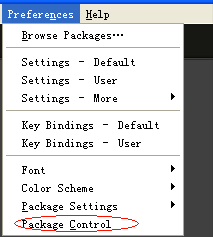
\includegraphics[width=8cm]{1.4.sublime3.png}
   \label{図1.7}
   \caption{sublimeパッケージ管理}
\end{figure}
  \item インストールが完了するとSublimeのプラグインをインストールできます。GoSublime, SidebarEnhancementsとGo Buildをインストールする必要があるので、プラグインをインストールしたあとSublimeを再起動させて有効にしてください。Ctrl+Shift+pでPackage Controlを開き、pcipを入力します。(これは"Package Control: Install Package"と省略されます)。\\ この時、左下のコーナーに現在読み込んでいるパッケージデータが表示されます。完了すると下のような画面になります。\\ 
\begin{figure}[H]
  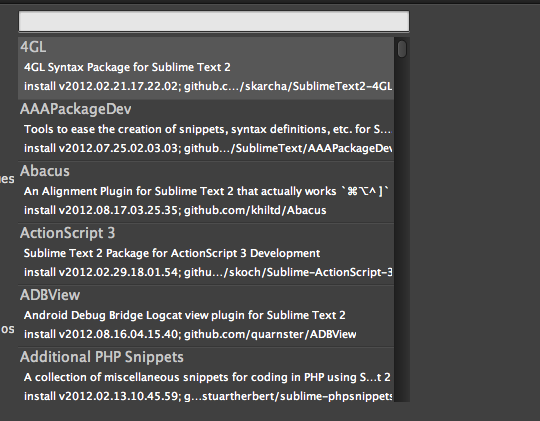
\includegraphics[width=14cm]{1.4.sublime4.png}
   \label{図1.8}
   \caption{sublimeプラグインのインストール画面}
\end{figure}
この時、GoSublimeと入力し、「確認」をクリックするとインストールが始まります。同じようにSidebarEnhancementsとGo Buildにも行います。
  \item インストールが成功したかテストします。Sublimeを開き、main.goを開いて文法がハイライトされているのをご確認ください。\texttt{import}を入力してコードの自動表示がされます。\texttt{import "fmt"}のあとに\texttt{fmt.}を入力すると自動的に関数の候補が現れます。\\ もしすでにこのような表示がされる場合は、インストールが成功しており、自動補完が完了しています。\\ もしこのような表示がなされない場合、あなたの\texttt{\$PATH}が正しく設定されていないのかもしれません。ターミナルを開き、gocodeを入力して、正しく実行できるか確認してください。もしダメであれば\texttt{\$PATH}が正しく設定されていません。 (XP向け)たまたまターミナルでの実行が成功することもあります。しかしsublimeは何も知らせてくれないかデコードエラーが発生します。sublime text3とconvert utf8プラグインを試してみてください。
  \item MacOSではすでに\$GOROOT, \$GOPATH, \$GOBINが設定されていても自動的にはどうすればよいか教えてくれません。\\ sublimeにてcommand + 9を押し、envを入力して\$PATH, \$GOROOT, \$GOPATH, \$GOBINといった変数を確認します。もしなければ、以下の手順に従ってください。\\まず下のシンボリックリンクを作成し、Terminalで直接sublimeを起動します
\begin{lstlisting}[numbers=none]
ln -s /Applications/Sublime\ Text\ 2.app/Contents/SharedSupport/
bin/subl /usr/local/bin/sublime
\end{lstlisting}
\end{enumerate}
